\chapter{Overview of Our Approach}
\label{chap.ourapproach}

In our research, we address focus on the lack of sophisticated algorithms that would help with automated testing during the MBD as described in \ref{sec:num3}. To our knowledge, for the higher level notations like Simulink, there are only algorithms which treat the models as a black box. The inner structure of the model is not taken into consideration in any way. We aim to create algorithms that will fill this gap and enhance the automated testing process of models of CPS by fully exploiting information stored in the structure of models. Our research plan is divided into goals:

\begin{itemize}
	\item Collaborate with the industry companies and gain access to models of CPS commonly used in practice
	\item Examine tools for automated testing of models of CPS and determine their drawbacks
	\item Develop new approaches and algorithms for automated testing of models of CPS
\end{itemize}

We have established a collaboration with czech company HUMUSOFT, spol. s r.o. Their areas of expertise include control systems, technical computing, model-based design and business process simulation. Activities of the company cover both development of own products and solutions and representing other IT companies offering complementary products and services on the local market. HUMUSOFT is a reseller of MathWorks, Inc., U.S.A., for the Czech Republic and Slovakia. They provide marketing and value added services for technical computing and simulation software MATLAB and Simulink.

We have acquired a model of EV powertrain test bench at Roztoky Science and Technology Park. The powertrain consists of a battery pack, a power inverter using DTC and an induction motor. For each of these components, there is a mathematical description, the methodology of system identication and a model validation by comparing simulation results with real device measurement. There is a control algorithm of the test bench to simulate the EV drive along a track with known altitude by the dened speed of the vehicle in respect to drive resistance forces. Control algorithm includes safety features to avoid test bench failure and is implemented in dSpace DS1103. The communication between actuators is established by the CAN communication protocol and the RS232 communication protocol.

We have joined our forces with Prof. Li Qiu from The Hong Kong University of Science and Technology and work together on a model of of Inverted Pendulum (iPendulum). The system consists of a cart and a rod. The cart, with a mass Mc, slides on a stainless steel shaft and is equipped with a motor. A rod, attached with a ball, is mounted on the cart whose axis of rotation is perpendicular to the direction of the motion of the cart. The rod has an evenly distributed mass Mp and a length L. The ball, with a mass Mb, can be regarded as a mass point. The card position x(t) and the pendulum angle theta(t) can be measured. The input is the force f(t) applied on the cart.

For our experiments we are using MATLAB/Simulink software (R2017b 64-bit), together with Stateflow package as described in {TODO add SotA chapter about it}. We use a cloud Windows Embedded 8 x64 OS with Intel(R) Xeon(R) CPU E5-2620 v3 @ 2.40Ghz and 8GB RAM. We measure performance of the S-TaLiRo tool during the falsification process for different models.

S-TaLiRo searches for trajectories of minimal robustness in Simulink/Stateflow simulations. It uses randomized testing based on stochastic optimalization techniques (Monte-Carlo, Ant-Colony optimalization, etc.). [Ant Colonies for Temporal Logic Falsification of Hybrid Systems Yashwanth Singh Rahul Annapureddy and Georgios E. Fainekos] It searches for counterexamples to Metric Temporal Logic (MTL) properties for CPS. This goal is achieved by a minimization of a robustness metric [Robustness of Temporal Logic Specifications for Finite State Sequences in Metric Spaces Georgios E. Fainekos and George J. Pappas]. In it's core S-TaLiRo uses combination of stochastic sampling together with Simulink simulation and a typically a certain form of optimalization. This way it aims to find the smallest robustness for a model which is desirable, because traces with lower robustness value are closer in distance to falsifying traces. If the tool detect a negative robustness we acquire a trace which falsify temporal logic properties. We refer to it as a witness trajectory. Robustness is calculated by TaLiRo module, but the computation is based on the results of convex optimalization problems used to compute signed distances.

In order to run different experiments on different CPS and other real-time systems we have to adapt to the usage of MTL in S-TaLiRo tools. Traditional MTL operators are used in S-TaLiRo MATLAB scripts according to \tabref{tab.MTLsTaLiRo}. For each of these operators we can also specify time bounds $[a,b\}$ where a and b are non-negative integer values and we use round bracket for b when b is infinity, else use TODO find the name of chlupata zavorka. Values of a,b are lower/upper bounds not on simulation time, but on the number of samples. The actual sample time constraints can be derived from the sampling value of the "Rate Transition" block. TODO: find what block it is.

\begin{table}[htb]
\begin{center}
\begin{tabular}{|p{9cm}|c|c|}
	\hline
	Language representation & MTL symbol & S-TaLiRo\\
	\hline
	not & MTL not & $!$ \\
	\hline	
	and & MTL and & /\textbackslash \\
	\hline
	or & MTL and & \textbackslash/ \\
	\hline
	if ... then ... & MTL &$\rightarrow$ \\
	\hline
	if and only if & MTL & $<->$ \\
	\hline
	it is always going to be the case & G (diamond) & $[ ]$ \\
	\hline
	at least once in the future & F (square) & $< >$ \\
	\hline
	it has always been the case & H & $[ . ]$ \\
	\hline
	at least once in the past & P & $< . >$ \\
	\hline
	phi will be true until a time when theta is true & until & U \\
	\hline
	phi has been true since a time when theta was true & since & S \\
	\hline
	phi has to hold at the next state & next & X \\
	\hline
	phi had to hold at the preceding state & previous & P \\
	\hline
\end{tabular}
\end{center}
\caption{Metric Temporal Logic operators in context of the S-TaLiRo tool.}
\label{tab.MTLsTaLiRo}
\end{table}

HERE talk about the models we used to run S-TaLiRo


The sample \figref{fig.float} shows ...

\begin{figure}[htb]
\begin{center}
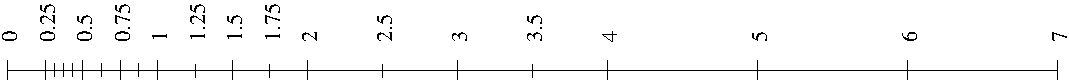
\includegraphics[width=.95\textwidth]{pic/float.pdf}
\end{center}
\caption{Distribution of the floating point numbers. This figure shows a distribution of a sample floating point number set with a precision $t=3$, and $e_{min}=-1$ and $e_{max}=3$.}
\label{fig.float}
\end{figure}


There are two basic floating point \index{Floating point} data types \index{Floating point!Data types}, as defined by the IEEE 754-2008 \cite{ieee754} standard, are shown in \tabref{tab.floatingpointdatatypes}.

\begin{table}[htb]
\begin{center}
\begin{tabular}{|r|c|c|c||c||c|}
% Draw horizontal table line from column 2 to column 6
% The first column is left empty, without the horizontal line
\cline{2-6}

% Since we do not want to change the formatting of the first column
% we need to use the multicolumn macro \multicolumn{#ofcolumns}{newformatting}{content}
% so we can change |r| to just r|. If we did not do that, we'd have the left
% vertical line drawn in the first column. Also in order to make the header row
% nicer, we use the \vrule macro. See below for an explanation.
\multicolumn{1}{r|}{} & {\vrule height 13pt depth 6pt width 0pt\bf Sign} [b] & {\bf Exponent} [b] & {\bf Mantissa} [b] & {\bf Prec.} [dig] & {\bf Total} [b]\\ \cline{2-6}  \hline

% This vrule shows that we can extend the column height or depth if necessary.
% This is useful for header rows or rows that contain some mathematical expressions.
\vrule height 10pt depth 20pt width 0pt
{\bf binary32}   			& 1    & 8        	& 24      & 8  	& 32\\ \hline

% To debug, make the vertical rule visible by specifying its width to 1 pt rather than 0 pt.
\vrule height 20pt depth 0pt width 1pt
{\bf binary64}   			& 1    & 11       	& 53      & 16	& 64\\ \hline
\end{tabular}
\end{center}
\caption{Basic floating point data types.}
\label{tab.floatingpointdatatypes}
\end{table}
